\documentclass[11pt,a4paper]{article}
\usepackage[margin=2.3cm]{geometry}
\usepackage[T1]{fontenc}
\usepackage{textcomp}
\input{glyphtounicode}
\pdfgentounicode=1
\usepackage{lmodern}
\usepackage{amsmath}
\usepackage{xcolor}
\usepackage{listings}
\usepackage{tcolorbox}
\usepackage{booktabs}
\usepackage{tikz}
\usepackage{hyperref}
\hypersetup{colorlinks=true, linkcolor=blue!50!black, citecolor=green!40!black}

\definecolor{codebg}{RGB}{248,248,245}
\lstset{
  language=C, basicstyle=\ttfamily\footnotesize, backgroundcolor=\color{codebg},
  keywordstyle=\color{blue!60!black}\bfseries, commentstyle=\color{green!45!black}\itshape,
  stringstyle=\color{red!60!black}, numbers=none, upquote=true,
  frame=single, rulecolor=\color{gray!40}, breaklines=true, columns=fullflexible,
  keepspaces=true, showstringspaces=false
}
\lstdefinestyle{sh}{language=bash, backgroundcolor=\color{black!5}}

\newtcolorbox{keyidea}{colback=blue!4, colframe=blue!45!black, title=Key ideas, fonttitle=\bfseries\small}
\newtcolorbox{experiment}{colback=orange!5, colframe=orange!70!black, title=Experiment, fonttitle=\bfseries\small}

\title{\textbf{OpenMP --- Lesson 4}\\[4pt]\large Sharing the work: the \texttt{for} construct}
\author{Gustavo Lozano}
\date{November 2026}

\begin{document}
\maketitle

\noindent\textit{\small Source: Chapman, Jost \& van der Pas~\cite{chapman}, Ch.~4
``OpenMP Language Features'' (the loop work-sharing construct and the combined
\texttt{parallel for}).}

\section{The idea}
In Lessons 1--3 every thread executed the \emph{whole} block, so with 4 threads the loop
ran 4 times. That shows how threads behave, but it does not make a program faster. To gain
speed, the threads must \textbf{divide} the work: each iteration of the loop is executed by
exactly \emph{one} thread. This is a \textbf{work-sharing} construct, and the most
important one is \texttt{for}.

\begin{center}
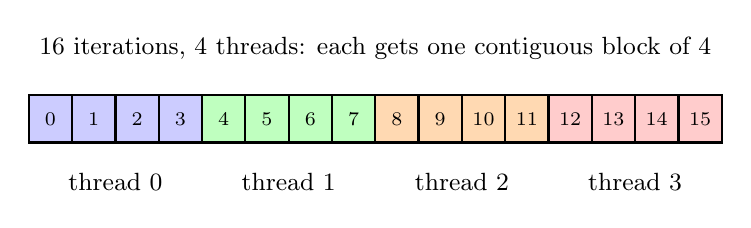
\begin{tikzpicture}[thick, x=0.55cm]
  \foreach \i in {0,...,15} {
    \pgfmathtruncatemacro{\t}{\i/4}
    \ifcase\t \def\c{blue!20}\or \def\c{green!25}\or \def\c{orange!30}\or \def\c{red!20}\fi
    \node[draw, fill=\c, minimum width=0.55cm, minimum height=0.6cm, font=\scriptsize] at (\i,0) {\i};
  }
  \foreach \t/\c in {0/blue!20,1/green!25,2/orange!30,3/red!20} {
    \node[font=\small] at (1.5+4*\t,-0.8) {thread \t};
  }
  \node[font=\small] at (7.5,0.9) {16 iterations, 4 threads: each gets one contiguous block of 4};
\end{tikzpicture}
\end{center}

\section{The syntax}
\begin{lstlisting}
#pragma omp parallel for          /* create a team AND split the next loop */
for (int i = 0; i < n; i++)
    work(i);
\end{lstlisting}
\begin{itemize}
  \item \texttt{parallel for} is a shortcut for a \texttt{parallel} region containing only
        an \texttt{omp for} loop.
  \item The loop index \texttt{i} is \textbf{private} automatically.
  \item There is an \textbf{implicit barrier} at the end of the loop: after it, all
        iterations are done.
  \item The loop must have a countable form (e.g.\ \texttt{for (i = a; i < b; i++)}),
        so OpenMP can compute the number of iterations before it starts.
  \item \textbf{You} must guarantee the iterations are \textbf{independent}. OpenMP does
        not check. Shared results are combined with \texttt{reduction} (Lesson~3).
\end{itemize}
How iterations are assigned to threads is called the \emph{schedule}. With the default
in GCC, each thread receives one contiguous block of about $n/p$ iterations. Other
schedules are the topic of Lesson~5.

\section{The example: computing $\pi$}
We use the identity
\[
  \pi = \int_0^1 \frac{4}{1+x^2}\,dx \;\approx\; h\sum_{i=0}^{n-1}\frac{4}{1+x_i^2},
  \qquad x_i = (i+\tfrac12)\,h,\quad h=\frac1n,
\]
(the midpoint rule). Each term depends only on $i$, so the iterations are independent,
and the only shared result, \texttt{sum}, is combined with \texttt{reduction(+:sum)}.

\section{The code}
\lstinputlisting[title=\texttt{parallel\_for.c}]{parallel_for.c}

\begin{lstlisting}[style=sh]
gcc -Wall -fopenmp -o parallel_for parallel_for.c
OMP_NUM_THREADS=4 ./parallel_for
\end{lstlisting}
Typical output (order and times will differ):
\begin{lstlisting}[style=sh]
  iteration  4 -> thread 1
  iteration  5 -> thread 1
  ...
  iteration  0 -> thread 0
  ...
  iteration 15 -> thread 3

threads = 4   pi = 3.141592653590   time = 0.1064 s
\end{lstlisting}

\begin{keyidea}
\begin{itemize}
  \item Each iteration runs exactly once, on one thread: the work is \emph{divided},
        not repeated.
  \item By default thread $k$ gets the $k$-th contiguous block of iterations.
  \item The printing order is still not deterministic, but the \emph{assignment}
        (which thread does which iteration) is fixed by the schedule.
  \item The value of $\pi$ is the same with any number of threads (up to rounding in the
        last digits, because floating-point addition is not associative and the
        reduction adds in a different order).
\end{itemize}
\end{keyidea}

\section{The experiment}
\begin{experiment}
\textbf{Question:} how much faster does the loop get as threads are added?
\begin{enumerate}
  \item Check your number of cores: \texttt{nproc}.
  \item Run the program with several thread counts. Keep only the last line:
\begin{lstlisting}[style=sh]
for t in 1 2 4 8; do OMP_NUM_THREADS=$t ./parallel_for | tail -1; done
\end{lstlisting}
  \item For each $p$ compute the \textbf{speed-up} and the \textbf{efficiency}:
        \[
          S(p) = \frac{T(1)}{T(p)}, \qquad E(p) = \frac{S(p)}{p}.
        \]
\end{enumerate}
\textbf{What to observe and answer.}
\begin{enumerate}
  \item In the ideal case $S(p)=p$. How close do you get while $p \le$ \texttt{nproc}?
  \item What happens to $S(p)$ when $p >$ \texttt{nproc}? Why?
  \item Why is $S(p)$ a bit below $p$ even when there are enough cores?
\end{enumerate}
\end{experiment}

\paragraph{Answers (read after trying).}
(1)~This loop is almost perfectly parallel: the iterations are independent and need no
synchronization. Expect $S(p)$ close to $p$; for example, on a 2-core machine
$T(1)=0.20$\,s and $T(2)=0.12$\,s give $S(2)\approx1.7$.
(2)~It stops growing. Once every core is busy, extra threads only take turns on the same
cores and add switching overhead. Threads are not cores (Lesson~1).
(3)~Creating the team, splitting the iterations, the barrier and the final reduction all
cost time that the serial program does not pay. This \emph{parallel overhead} is small
here, but it is never zero.

\paragraph{Next lesson.} The \texttt{schedule} clause: \texttt{static}, \texttt{dynamic} and
\texttt{guided}, and why the default split fails when iterations do unequal amounts of work
(Chapman et al., Ch.~4).

\begin{thebibliography}{9}
\bibitem{chapman} B.~Chapman, G.~Jost, and R.~van der Pas. \emph{Using OpenMP: Portable
  Shared Memory Parallel Programming}. MIT Press, Cambridge, MA, 2007.
\end{thebibliography}
\end{document}
